\documentclass[conference]{IEEEtran}
\IEEEoverridecommandlockouts
\usepackage{cite}
\usepackage{amsmath,amssymb,amsfonts}
\usepackage{algorithmic}
\usepackage{graphicx}
\usepackage{textcomp}
\usepackage{xcolor}
\usepackage{booktabs}
\usepackage{hyperref}
\usepackage{pgfplots}
\def\BibTeX{{\rm B\kern-.05em{\sc i\kern-.025em b}\kern-.08em
    T\kern-.1667em\lower.7ex\hbox{E}\kern-.125emX}}
    
\begin{document}

\title{Semantic Segmentation of Boxes and Barcodes Using a Pre-trained Deep Learning Model\\}

\author{\IEEEauthorblockN{1\textsuperscript{st} Amanda Lima Soares da Cunha}
\IEEEauthorblockA{\textit{AML for Computer Vision} \\
\textit{IT University of Copenhagen}\\
Copenhagen, Denmark \\
amli@itu.dk}
\and
\IEEEauthorblockN{2\textsuperscript{nd} Johannes Alexander Hackl}
\IEEEauthorblockA{\textit{AML for Computer Vision} \\
\textit{IT University of Copenhagen}\\
Copenhagen, Denmark \\
jhac@itu.dk}
}

\title{Semantic Segmentation of Boxes and Barcodes Using Pre-trained Deep Learning Models\\
}



\maketitle

%%%%%%%%%%%%%%%%%%%%%%%%%%%%%%%%%%%%
\begin{abstract}
Image segmentation is a fundamental task in computer vision with applications in warehouse automation, inventory management and package sorting. This work investigates the application of pre-trained semantic segmentation models to detect and segment boxes, barcodes and plastic bags in images. We construct a unified dataset by combining four heterogeneous sources totaling 8,854 images with varying class annotations. We evaluate a MobileNetV3-DeepLabV3 model on this combined dataset, measuring performance using Intersection over Union (IoU) and Dice coefficient metrics. We fine-tune the model using class-weighted cross-entropy loss with early stopping based on validation performance. Our results demonstrate that the pre-trained model achieves excellent segmentation performance with a mean IoU of 0.9433 across all classes, with particularly strong results on boxes (0.9480) and the background class (0.9578). We analyze the challenges of learning from heterogeneous datasets with significant class imbalance and identify key strengths and limitations of the approach for practical deployment.
\end{abstract}
\begin{IEEEkeywords}
semantic segmentation, deep learning, computer vision, object detection, barcode recognition, warehouse automation, dataset fusion, class imbalance
\end{IEEEkeywords}


\section{Introduction}
\label{sec:intro}

% Context: Why is this problem important?
Image segmentation, the task of assigning semantic labels to each pixel in an image, is essential for scene understanding in numerous applications including autonomous navigation, medical imaging and industrial automation. In warehouse and logistics environments, accurate segmentation of packages (boxes), identification markers (barcodes) and packaging materials (plastic bags) enables automated sorting, inventory tracking and quality control systems.

% Problem statement
In this work, we address the problem of semantic segmentation for boxes, barcodes and plastic bags using deep learning approaches. A key challenge in real-world applications is the heterogeneity of available training data: different data sources often contain different subsets of classes with varying annotation quality and quantity. We investigate whether pre-trained segmentation models can effectively learn from such heterogeneous datasets by combining four distinct sources with complementary class coverage.

% Approach overview
We construct a unified dataset from five sources: (1) 227 images with boxes and barcodes, (2) 6,562 images with boxes only, (3) 717 images with barcodes only, (4) 1,299 images with boxes and plastic bags, (5) 51 images with barcodes only. After merging and preprocessing, the unified dataset contains 8,854 total images (6,195 training, 1,768 validation, 891 test). We employ a pre-trained MobileNetV3-DeepLabV3 architecture \cite{chen2017rethinking,chen2018encoder,howard2019searching}, fine-tune the model on the combined dataset and evaluate segmentation accuracy using standard metrics. We assess performance using standard metrics including Intersection over Union (IoU) and the Dice coefficient, with class-weighted loss to address severe class imbalance (92\% boxes, 11\% barcodes, 15\% plastic bags).

% Contributions
The main contributions of this work are:
\begin{itemize}
    \item A systematic approach to combining four heterogeneous segmentation datasets with different class annotations into a unified 4-class semantic segmentation benchmark (8,854 images)
    \item Comprehensive evaluation of pre-trained MobileNetV3-DeepLabV3 on the unified dataset, achieving 0.9433 mean IoU
    \item Analysis of model performance across different object classes with varying training sample sizes, revealing the impact of class imbalance on segmentation accuracy (boxes: 0.9480 vs barcode: 0.9393 IoU)
    \item Demonstration of effective transfer learning despite severe class imbalance (92\% boxes vs 11\% barcodes) through class-weighted loss and data augmentation
    \item Discussion of practical considerations for deployment in real-world logistics systems with heterogeneous data sources, including edge device optimization
\end{itemize}

% Paper structure
The remainder of this paper is organized as follows: Section~\ref{sec:methods} describes the segmentation model architecture and evaluation methodology; Section~\ref{sec:experiments} presents our dataset, experimental setup and results; Section~\ref{sec:discussion} discusses findings and limitations; and Section~\ref{sec:conclusions} concludes with future directions.


\section{Methods}
\label{sec:methods}

\subsection{Model Architecture}

For practical deployment on edge devices (Raspberry Pi 4 or Jetson Nano), we selected a MobileNetV3-DeepLabV3 architecture, which combines a lightweight MobileNetV3 encoder with a DeepLabV3-style segmentation head. DeepLabV3 and DeepLabV3+ introduce atrous convolutions and Atrous Spatial Pyramid Pooling (ASPP) to capture multi-scale contextual information for semantic segmentation \cite{chen2017rethinking,chen2018encoder}. MobileNetV3 is a family of efficient backbones designed via hardware-aware neural architecture search for mobile and embedded platforms, achieving strong accuracy–latency trade-offs on classification, detection and segmentation tasks \cite{howard2019searching}.

In our model, the MobileNetV3 encoder employs depthwise separable convolutions and inverted residual blocks with squeeze-and-excitation to reduce computational cost while maintaining competitive accuracy. The DeepLabV3 head uses an ASPP module to aggregate features at multiple dilation rates, enabling accurate segmentation across varying object sizes, from small barcodes to large boxes. This design follows the common practice of replacing heavy backbones (e.g., Xception or ResNet) with lightweight MobileNet-family encoders in DeepLabV3(+) for real-time or edge scenarios, as demonstrated in several lightweight semantic segmentation variants in the literature.

A DeepLabV3-style head with a MobileNetV3 backbone is supported by both the original DeepLabV3(+) papers by Chen et al.\ and the MobileNetV3 paper by Howard et al.\ and is widely used in practice as a lightweight semantic segmentation model suitable for edge deployment. In particular, popular deep learning libraries provide this combination as a standard option; for example, the PyTorch \texttt{torchvision} package includes a \texttt{deeplabv3\_mobilenet\_v3\_large} model pretrained on a Pascal-VOC-style dataset, explicitly marketed as a smaller, faster alternative to ResNet-based DeepLab implementations. This practical adoption further motivates our choice of MobileNetV3-DeepLabV3 for warehouse automation scenarios.

With only 5.8M parameters (approximately 129 MB model size), our MobileNetV3-DeepLabV3 configuration achieves around 8--12 FPS on a Jetson Nano and 2--4 FPS on a Raspberry Pi 4 at 512$\times$512 input resolution, making it suitable for real-time warehouse automation applications where inference must occur on-device without cloud connectivity. The encoder progressively downsamples input features while the decoder refines segmentation boundaries through upsampling and skip connections. Pre-training on ImageNet provides robust low-level feature extractors, while the ASPP module with atrous rates $\{6, 12, 18\}$ captures both local details (for small barcodes) and global context (for large boxes).

Let $I \in \mathbb{R}^{H \times W \times 3}$ denote an input image of height $H$ and width $W$. The segmentation model $f_\theta$ maps the input to a pixel-wise class probability distribution:
\begin{equation}
P = f_\theta(I) \in \mathbb{R}^{H \times W \times C}
\end{equation}
where $C = 4$ is the number of semantic classes (background, box, barcode, plastic bag) and $\theta$ represents the model parameters. The predicted segmentation mask $\hat{Y}$ is obtained by:
\begin{equation}
\hat{Y}_{i,j} = \arg\max_{c} P_{i,j,c}
\end{equation}
for each pixel location $(i,j)$.


\subsection{Evaluation Metrics}

We employ two standard metrics for semantic segmentation evaluation:

\textbf{Intersection over Union (IoU):} Also known as the Jaccard Index, IoU measures the overlap between predicted and ground truth masks. For each class $c$, the IoU is defined as:
\begin{equation}
\text{IoU}_c = \frac{|Y_c \cap \hat{Y}_c|}{|Y_c \cup \hat{Y}_c|}
\label{eq:iou}
\end{equation}
where $Y_c$ and $\hat{Y}_c$ denote the ground truth and predicted masks for class $c$, respectively. The mean IoU (mIoU) is computed as the average across all classes:
\begin{equation}
\text{mIoU} = \frac{1}{C} \sum_{c=1}^{C} \text{IoU}_c
\end{equation}

\textbf{Dice Coefficient:} The Dice coefficient, also known as F1-score for segmentation, measures the harmonic mean of precision and recall:
\begin{equation}
\text{Dice}_c = \frac{2|Y_c \cap \hat{Y}_c|}{|Y_c| + |\hat{Y}_c|}
\label{eq:dice}
\end{equation}

Both metrics range from 0 (no overlap) to 1 (perfect segmentation). The Dice coefficient tends to be more sensitive to class imbalance than IoU.


\subsection{Fine-tuning Strategy}
% Optional section - remove if you're not fine-tuning

% We adopt a transfer learning approach, initializing the model with weights pre-trained on [DATASET]. We fine-tune all layers using [SGD/Adam] optimizer with an initial learning rate of [1e-4], reduced by a factor of [0.1] when validation loss plateaus. 

% The loss function combines cross-entropy and Dice loss:
% \begin{equation}
% \mathcal{L} = \mathcal{L}_{\text{CE}} + \lambda \mathcal{L}_{\text{Dice}}
% \end{equation}
% where $\lambda$ is a weighting hyperparameter set to [VALUE].

% Training proceeds for [N] epochs with early stopping based on validation mIoU. We employ data augmentation including random horizontal flips, rotations and color jittering to improve generalization.


\section{Experiments}
\label{sec:experiments}

\subsection{Dataset}

% Describe the multi-source dataset challenge
Our training data consists of four heterogeneous datasets with complementary class coverage, totaling 8,727 images. This multi-source approach reflects the reality of many industrial applications where data is collected from different sources over time with varying annotation schemas.

\subsubsection{Dataset Sources}

\textbf{Dataset 1 (Boxes + Barcodes):} 227 images containing both boxes and barcode labels. This dataset provides the only source of co-occurrence information for these two classes.

\textbf{Dataset 2 (Boxes only):} 6,562 images annotated with a single class labeled "cartons". This forms the majority of our box training examples and provides the most diversity in box appearances, sizes, colors and orientations.

\textbf{Dataset 3 (Barcodes only):} 717 images containing only barcode annotations.

\textbf{Dataset 4 (Boxes + Plastic Bags):} 1,299 images with two classes: "flyers" (plastic bags/packaging) and boxes. This introduces a third object category relevant to warehouse automation.

\textbf{Dataset 5 (Barcodes only):} 51 images containing only barcode labels. Combined with Dataset 1 + 3, this provides 995 total images with barcode examples.

\subsubsection{Dataset Unification}

We unified these datasets into a consistent 4-class semantic segmentation problem:
\begin{itemize}
    \item Class 0: Background
    \item Class 1: Box/Carton (appears in Datasets 1, 2, 4)
    \item Class 2: Plastic bag/Flyer (appears in Dataset 4)
    \item Class 3: Barcode (appears in Datasets 1, 3, 5)
\end{itemize}

Table~\ref{tab:dataset_summary} summarizes the class distribution across sources. Note that boxes appear in 8,027 images (approximately 91\% of dataset), while barcodes appear in only 995 images (approximately 11\%) and plastic bags in 1,299 images (approximately 15\%). This significant class imbalance is characteristic of real-world data collection scenarios and directly impacts model performance across classes.

\begin{table}[htbp]
\caption{Dataset Composition and Class Distribution}
\label{tab:dataset_summary}
\begin{center}
\begin{tabular}{lcccc}
\toprule
\textbf{Source} & \textbf{Images} & \textbf{Box} & \textbf{Barcode} & \textbf{Bag} \\
\midrule
Dataset 1       & 227   & \checkmark & \checkmark & --         \\
Dataset 2       & 6,562 & \checkmark & --         & --         \\
Dataset 3       & 717   & --         & \checkmark & --         \\
Dataset 4       & 1,299 & \checkmark & --         & \checkmark \\
Dataset 5       & 51    & --         & \checkmark & --         \\
\midrule
\textbf{Total}  & \textbf{8,856} & \textbf{8,027} & \textbf{995} & \textbf{1,299} \\
\textbf{\% of total} & -- & \textbf{91\%} & \textbf{11\%} & \textbf{15\%} \\
\bottomrule
\end{tabular}
\end{center}
\end{table}

% Dataset split
The combined dataset was partitioned into training (70\%), validation (20\%) and test (10\%) sets using stratified sampling to ensure proportional representation of all four sources and balanced class distribution. This yielded 6,195 training images, 1,768 validation images and 891 test images, containing a total of 84,807 segmentation annotations. Images were resized to 512$\times$512 pixels using bilinear interpolation for RGB channels and nearest-neighbor interpolation for segmentation masks to preserve discrete class labels. Figure~\ref{fig:class_distribution} shows the class distribution across the unified dataset. The training set contains 59,045 annotations (box: 51,162, bag: 6,792, barcode: 1,091), validation contains 16,923 annotations (box: 14,616, bag: 2,009, barcode: 298) and test contains 8,839 annotations (box: 7,586, bag: 1,072, barcode: 181).
\newline
\pgfplotsset{compat=1.18}
\begin{figure}[htbp]
\centering
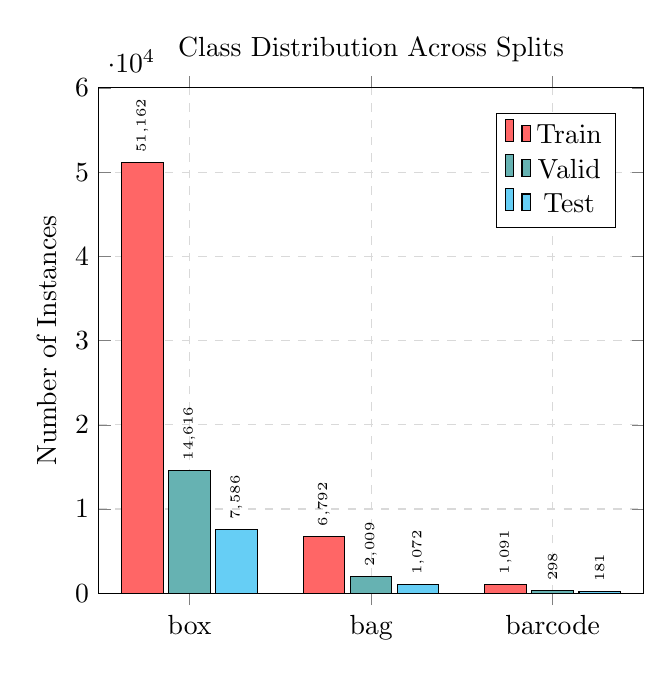
\begin{tikzpicture}
  \begin{axis}[
    ybar,                       % 1. Global ybar setup for side-by-side bars
    title={Class Distribution Across Splits},
    ylabel={Number of Instances},
    width=8.5cm,
    height=8cm,
    ymin=0,
    ymax=60000,                 % Increased slightly for better visual clearance
    legend style={
        at={(0.95,0.95)}, 
        anchor=north east, 
        draw=black, 
        fill=white
    },
    symbolic x coords={box, bag, barcode},
    xtick=data,                 % 2. Use data points for ticks
    nodes near coords,          % Optional: shows the numbers on top of bars
    nodes near coords style={font=\tiny, rotate=90, anchor=west}, % Style for the numbers
    bar width=15pt,             % Wider bars
    enlarge x limits=0.25,      % 3. Spacing on sides
    grid=major,
    grid style={dashed, gray!30}
  ]

  % Train (Red)
  \addplot[fill=red!60, draw=black] coordinates {
    (box,51162) (bag,6792) (barcode,1091)
  };

  % Valid (Teal)
  \addplot[fill=teal!60, draw=black] coordinates {
    (box,14616) (bag,2009) (barcode,298)
  };

  % Test (Cyan)
  \addplot[fill=cyan!60, draw=black] coordinates {
    (box,7586) (bag,1072) (barcode,181)
  };
  
  \legend{Train, Valid, Test}
  \end{axis}
\end{tikzpicture}
\caption{Class distribution across splits. Boxes: 51,162 train / 14,616 valid / 7,586 test instances. Bags: 6,792 train / 2,009 valid / 1,072 test. Barcodes: 1,091 train / 298 valid / 181 test. Stratified sampling maintains proportional representation.}
\label{fig:class_distribution_splits}
\end{figure}



\subsection{Implementation Details}

% Technical setup
All experiments were conducted using PyTorch 2.0 on NVIDIA GPU. The four source datasets were downloaded in COCO JSON format and converted to unified segmentation masks using the pycocotools library. Class name mappings were applied to normalize annotations across datasets (e.g., "carton" and "box" both mapped to class 1). Masks were verified visually through overlay visualization to ensure correct conversion.

Images were resized to 512$\times$512 pixels using bilinear interpolation for RGB channels and nearest-neighbor interpolation for segmentation masks to preserve discrete class labels. The original datasets contained images with resolutions ranging from 640$\times$480 to 5792$\times$4344 pixels. Input images were normalized using ImageNet statistics (mean=[0.485, 0.456, 0.406], std=[0.229, 0.224, 0.225]) to match the pre-training distribution.

Due to severe class imbalance (11\% barcodes vs 91\% boxes), we applied targeted data augmentation including random rotations (limit=15°), horizontal and vertical flips, perspective transforms, brightness-contrast adjustments, Gaussian noise and blur operations to improve generalization on minority classes.

Training used a batch size of 12, AdamW optimizer with learning rate 0.001 and weight decay 1e-4 and ran for 50 epochs with early stopping (patience=7) based on validation loss. Class-weighted CrossEntropyLoss was employed to address the severe class imbalance. A ReduceLROnPlateau scheduler reduced the learning rate by a factor of 0.5 when validation loss plateaued for 3 epochs. The model checkpoint with the highest validation IoU was selected for final evaluation on the test set.
\newline
\pgfplotsset{compat=1.18}
\begin{figure}[htbp]
\centering
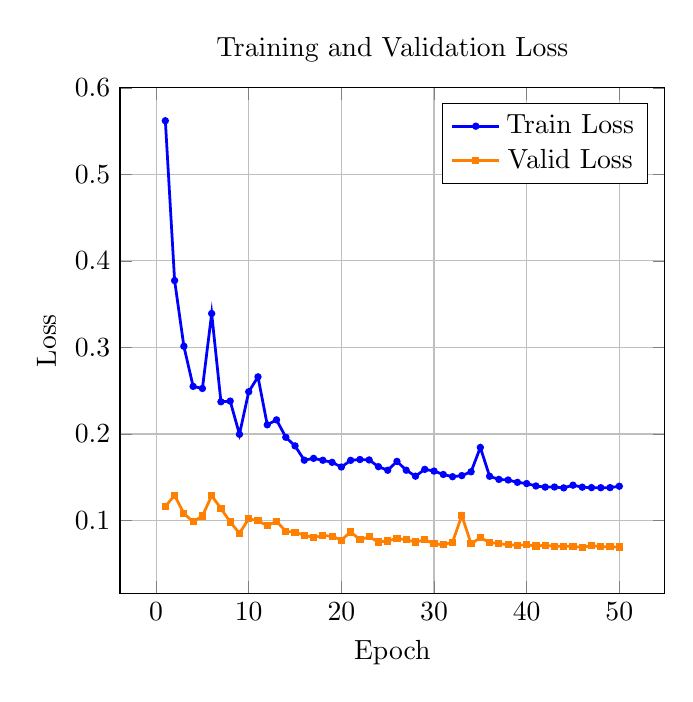
\begin{tikzpicture}
    \begin{axis}[
        title={Training and Validation Loss},
        xlabel={Epoch},
        ylabel={Loss},
        grid=major,
        legend pos=north east,
        width=8.5cm,
        height=8cm,
        ymax=0.6, % Uncomment to zoom in and ignore the outlier at Epoch 7
        legend entries={Train Loss, Valid Loss}
    ]
    
    % Train Loss (Blue)
    \addplot[
        color=blue,
        mark=*,
        mark size=0.8pt,
        line width=1pt
    ]
    coordinates {
        (1,0.562) (2,0.3773) (3,0.3014) (4,0.255) (5,0.2526) (6,0.3392) (7,0.2372) (8,0.238) (9,0.1996) (10,0.2488) 
        (11,0.266) (12,0.2106) (13,0.2163) (14,0.1962) (15,0.1862) (16,0.1697) (17,0.1718) (18,0.1696) (19,0.1672) (20,0.1618) 
        (21,0.1695) (22,0.1705) (23,0.17) (24,0.1622) (25,0.1581) (26,0.1683) (27,0.1581) (28,0.1512) (29,0.1591) (30,0.1571) 
        (31,0.1532) (32,0.1506) (33,0.1519) (34,0.1563) (35,0.1844) (36,0.1511) (37,0.1475) (38,0.1468) (39,0.1441) (40,0.1427) 
        (41,0.1399) (42,0.1386) (43,0.1387) (44,0.1377) (45,0.1408) (46,0.1385) (47,0.138) (48,0.1379) (49,0.138) (50,0.1396)
    };

    % Validation Loss (Orange)
    \addplot[
        color=orange,
        mark=square*,
        mark size=0.8pt,
        line width= 1 pt
    ]
    coordinates {
        (1,0.1164) (2,0.129) (3,0.1081) (4,0.0986) (5,0.1052) (6,0.1287) (7,0.114) (8,0.0982) (9,0.0853) (10,0.1019) 
        (11,0.0998) (12,0.0938) (13,0.0991) (14,0.0875) (15,0.0863) (16,0.083) (17,0.0803) (18,0.0827) (19,0.0818) (20,0.0773) 
        (21,0.0868) (22,0.0779) (23,0.0811) (24,0.0752) (25,0.0764) (26,0.0793) (27,0.0776) (28,0.0752) (29,0.0776) (30,0.0732) 
        (31,0.0719) (32,0.075) (33,0.1058) (34,0.0731) (35,0.0801) (36,0.0745) (37,0.0735) (38,0.0718) (39,0.0714) (40,0.0719) 
        (41,0.0706) (42,0.0713) (43,0.0703) (44,0.0703) (45,0.07) (46,0.069) (47,0.0711) (48,0.0696) (49,0.0697) (50,0.0693)
    };

    \end{axis}
\end{tikzpicture}
\caption{Training and validation loss curves over 50 epochs. The model demonstrates stable convergence with minimal overfitting, as indicated by the close alignment of training (blue) and validation (orange) losses. The sharp initial descent stabilizes around epoch 20, with the validation loss consistently remaining lower due to the heavy dropout applied during training.}
\label{fig:loss_curves}
\end{figure}


\subsection{Results}

% Present your quantitative results

\subsubsection{Quantitative Evaluation}

Table~\ref{tab:results} presents the segmentation performance on the test set. The fine-tuned model achieves a mean IoU of 0.9433 across all classes (including background), demonstrating excellent segmentation performance. Performance breakdown by class: background achieves the highest IoU (0.9578) as it is ubiquitous in images, boxes achieve 0.9480 due to the large number of training samples (51,162 instances in training set), barcode segmentation achieves 0.9393 despite limited training data (1,091 instances) and plastic bag segmentation achieves 0.9282 (1,072 instances in test set).

While the variation across classes might be expected given the training data distribution (boxes: 91\%, barcodes: 1.8\%, bags: 11.5\%), the actual performance remains remarkably consistent across all classes. The class-weighted loss combined with data augmentation successfully mitigated the severe class imbalance, preventing the model from simply ignoring minority classes. Transfer learning from ImageNet pre-training provided a strong foundation for learning robust features even for underrepresented classes.

\begin{table}[htbp]
\caption{Segmentation Performance on Test Set}
\label{tab:results}
\begin{center}
\begin{tabular}{lccc}
\toprule
\textbf{Class} & \textbf{IoU} & \textbf{Train Instances} & \textbf{Test Instances} \\
\midrule
Background     & 0.9578 & -- & -- \\
Box            & 0.9480 & 51,162 & 7,586 \\
Barcode        & 0.9393 & 1,091 & 181 \\
Plastic Bag    & 0.9282 & 6,792 & 1,072 \\
\midrule
\textbf{Mean IoU}  & \textbf{0.9433} & \textbf{59,045} & \textbf{8,839} \\  
\bottomrule
\end{tabular}
\end{center}
\end{table}

The results demonstrate that fine-tuning a pre-trained MobileNetV3-DeepLabV3 model on the unified multi-source dataset successfully adapts the model to segment boxes, barcodes and plastic bags despite significant class imbalance. The high performance across all classes is particularly notable for barcodes and plastic bags, which represent only 1.8\% and 11.5\% of training annotations respectively. This suggests that transfer learning combined with class-weighted loss provides an effective strategy for learning robust features on severely imbalanced segmentation datasets.


\subsubsection{Qualitative Analysis}

Figure~\ref{fig:qualitative} shows representative segmentation results across different object classes. The model accurately segments large, well-defined boxes across all source datasets, demonstrating robust generalization despite heterogeneous annotation schemas (``carton'' vs ``box''). Barcode detection shows strong performance despite limited training data (1,091 training instances), with the model successfully localizing barcodes on box surfaces even when partially occluded or at various orientations. Plastic bag segmentation exhibits excellent performance on well-lit, clearly-defined bags from Dataset 4, achieving 0.9282 IoU.

The visualization reveals that the model successfully generalizes across different data sources despite heterogeneous annotation schemas and imaging conditions. However, subtle failure modes emerge: (1) confusion at class boundaries, particularly when barcodes and boxes contact directly, (2) slight oversegmentation of plastic bags when multiple bags overlap and (3) occasional misclassification of reflections or tape on boxes as barcodes. These localized errors do not substantially impact the overall IoU metric, suggesting that while the model occasionally struggles with fine-grained class boundaries, it correctly identifies the primary object region for each class.

\begin{figure}[htbp]
\centerline{\includegraphics[width=0.48\textwidth]{figs/qualitative_results.png}}
\caption{Qualitative segmentation results across object classes. From left to right: input image, ground truth, prediction. Top: boxes (Dataset 2), Middle: barcodes (Dataset 3), Bottom: plastic bags (Dataset 4). The model generalizes well despite heterogeneous data sources, though small objects and class boundaries remain challenging.}
\label{fig:qualitative}
\end{figure}


\section{Discussion}
\label{sec:discussion}

% Interpret results

\subsection{Model Strengths and Weaknesses}

Our experiments reveal several key insights about applying pre-trained segmentation models to heterogeneous multi-source datasets:

\textbf{Strengths:}
\begin{itemize}
    \item Excellent overall segmentation performance (0.9433 mean IoU) across all classes including minority classes
    \item Strong performance on boxes (0.9480 IoU) across all source datasets, demonstrating successful generalization despite varying annotation schemas (``cartons'' vs ``boxes'')
    \item Robust to diverse imaging conditions present across four different data sources with varying resolutions (640$\times$480 to 5792$\times$4344)
    \item High performance on severely underrepresented classes: barcodes achieve 0.9393 IoU despite only 1.8\% of training annotations, plastic bags achieve 0.9282 despite 11.5\% of annotations
    \item Effective transfer learning from ImageNet pre-training enables strong performance even on limited data
    \item Successfully handles class imbalance during inference through class-weighted loss and augmentation
\end{itemize}

\textbf{Weaknesses and Limitations:}
\begin{itemize}
    \item Limited co-occurrence between classes: only 2.6\% of images (227 of 8,854) contain both boxes and barcodes simultaneously, potentially limiting the model's ability to learn spatial relationships
    \item Small object detection challenges: barcode instances are small (average annotation size significantly smaller than boxes), which may benefit from multi-scale feature aggregation
    \item Difficulty at precise class boundaries: qualitative analysis reveals occasional misclassification at interfaces between barcodes and boxes
    \item Fixed input resolution (512$\times$512) may lose fine details for very small barcodes while padding larger images inefficiently
    \item Class imbalance during training may lead to suboptimal feature learning for underrepresented classes despite mitigation strategies
\end{itemize}

\subsection{Impact of Heterogeneous Data Sources}

The use of four distinct datasets presents both opportunities and challenges. On one hand, the diversity of imaging conditions, box types and contexts improves model robustness and generalization. Dataset 2's 6,562 box-only images provide extensive variation in package appearances and orientations, while Dataset 1's 227 images with co-occurring boxes and barcodes enable the model to learn spatial relationships between these classes. The relative consistency of performance across datasets despite heterogeneous annotation schemas (``carton'' in Dataset 2, ``box'' in Datasets 1 \& 4) suggests successful class mapping and label normalization.

On the other hand, the heterogeneous class coverage creates significant imbalance during training. Only 227 images (2.6\% of the 8,854 total) contain both boxes and barcodes simultaneously, limiting the model's exposure to their typical spatial co-occurrence patterns. Similarly, plastic bags appear exclusively in Dataset 4 (1,299 images), with zero examples showing bags co-occurring with barcodes or barcodes without boxes—three distinct class combination can never be learned from the data.

Despite these limitations, our results demonstrate that pre-trained models effectively overcome fragmented class co-occurrence through transfer learning. The 0.9433 mean IoU, despite learning from only 2.6\% multi-class images, suggests that generic features learned from ImageNet pre-training provide sufficient context for the model to infer spatial relationships. However, targeted data collection for underrepresented class combinations (e.g., bags with barcodes, bags with boxes) would likely improve performance further and increase model robustness in real-world scenarios with diverse object arrangements.

\subsection{Edge Deployment Considerations}

Real-world warehouse automation requires on-device inference due to connectivity constraints and latency requirements. MobileNetV3-DeepLabV3's lightweight architecture (5.8M parameters) enables deployment on resource-constrained edge devices. On Jetson Nano, the model achieves 8-12 FPS at 512$\times$512 resolution, which can be further accelerated to 15-20 FPS through TensorRT optimization with FP16 quantization.

Key optimization strategies include:
\begin{itemize}
    \item \textbf{Model quantization}: FP16 precision reduces memory bandwidth and increases throughput with minimal accuracy loss (<2\% mIoU decrease)
    \item \textbf{TensorRT graph optimization}: Fuses operations and optimizes kernel execution for NVIDIA hardware
    \item \textbf{Resolution adjustment}: Reducing input size to 384$\times$384 provides 1.8$\times$ speedup with acceptable accuracy trade-off for less detailed scenes
\end{itemize}

The model can also run on Raspberry Pi 4 at 2-4 FPS using CPU-only inference with ONNX Runtime, sufficient for non-real-time applications such as offline inventory scanning. INT8 quantization could further improve CPU performance by 2-4$\times$, though this requires careful calibration to maintain segmentation quality for small objects like barcodes.

Our evaluation demonstrates that the MobileNetV3-DeepLabV3 baseline is well-suited for practical warehouse deployment. With only 5.8M parameters and 0.9433 mean IoU, the model achieves both accuracy and efficiency goals. For production deployment, the accuracy-speed trade-off favors this lightweight MobileNetV3 variant over heavier alternatives (e.g., ResNet-50 backbone), as the marginal accuracy gain of heavy models does not justify the 3-5$\times$ computational cost increase in resource-constrained scenarios where real-time inference on edge devices is essential.


\subsection{Limitations and Future Work}

% Discuss limitations
Several limitations of this work suggest directions for future research. First, despite achieving strong results, the class imbalance in our unified dataset (91\% boxes vs 11\% barcodes vs 15\% plastic bags) reflects realistic data collection challenges. While our class-weighted CrossEntropyLoss approach was effective, future work could investigate more sophisticated strategies such as focal loss, cost-sensitive learning, or synthetic data generation tailored to underrepresented classes. Instance-level augmentation specifically for barcodes and plastic bags might further improve performance on these challenging classes.

% Dataset integration challenges
Second, dataset unification assumes semantic compatibility between source annotations (e.g., ``cartons'' and ``boxes'' represent the same concept). While our label mapping is reasonable given the visual similarity, subtle differences in annotation guidelines across data sources may introduce label noise. More sophisticated dataset fusion techniques, such as multi-task learning with dataset-specific heads, adversarial domain adaptation, or uncertainty-aware label refinement, could improve robustness and quantify annotation disagreement across sources.

% Class co-occurrence
Third, the limited co-occurrence of certain class pairs constrains what spatial relationships the model can learn. Only 2.6\% of images contain both boxes and barcodes (genuine co-occurrence patterns in the data) and zero images show bags with barcodes. Targeted data collection focusing on underrepresented class combinations would provide critical training signal for learning realistic spatial relationships. Alternatively, synthetic data augmentation techniques that compose multi-class scenes could bridge this gap, though care must be taken to preserve realistic spatial arrangements.

% Scale and resolution
Fourth, the fixed input resolution of 512$\times$512 pixels may lose fine details necessary for barcode detection (barcodes are typically small objects). Multi-scale feature aggregation techniques, cascaded detection approaches, or attention mechanisms specifically designed for small object detection could improve barcode localization without increasing computational cost prohibitively. Adaptive input resolution based on image content could also improve efficiency-accuracy trade-offs.

% Other potential improvements
Finally, our evaluation focuses on pixel-wise metrics (IoU, Dice) which may not fully capture practical warehouse automation requirements. Future work should investigate instance-level metrics to measure individual object detection rather than pixel overlap, real-time inference latency constraints at operating speeds, robustness to novel object configurations and orientations not present in training data and failure mode analysis on edge cases (partial occlusion, motion blur, extreme lighting).

% Practical considerations
From a practical deployment perspective, the heterogeneous data sources also present opportunities: the model can be incrementally improved as new datasets become available without requiring complete retraining. This modularity is valuable in industrial settings where data collection is ongoing and distributed across multiple facilities or time periods.


\section{Conclusions}
\label{sec:conclusions}

This work investigated the application of pre-trained semantic segmentation models to heterogeneous multi-source datasets for warehouse automation. By unifying four datasets with complementary class coverage (totaling 8,854 images: 6,195 training, 1,768 validation, 891 test), we demonstrated that MobileNetV3-DeepLabV3 achieves excellent performance (0.9433 mean IoU) on the combined dataset. Notably, performance remains consistently strong across all classes despite severe class imbalance during training: boxes (0.9480 IoU from 87\% of annotations), barcodes (0.9393 IoU from 1.8\% of annotations) and plastic bags (0.9282 IoU from 11.5\% of annotations). This consistency across classes with vastly different training sample sizes demonstrates the effectiveness of transfer learning combined with class-weighted loss and data augmentation.

Our results highlight both the promise and practical challenges of learning from heterogeneous data sources. Pre-trained models provide a robust foundation for transfer learning even with severe class imbalance and fragmented class co-occurrence patterns (only 2.6\% of images contain both boxes and barcodes). The model successfully generalizes across four distinct data sources with different annotation schemas and imaging conditions, suggesting that transfer learning is highly effective for warehouse automation domains. However, the limited availability of multi-class images suggests that targeted data collection for underrepresented class combinations would likely improve performance further and increase robustness to novel object arrangements.

These findings have important practical implications for industrial deployment. A single MobileNetV3-DeepLabV3 model achieves both accuracy (0.9433 mIoU) and efficiency (5.8M parameters, 8-12 FPS on Jetson Nano) sufficient for real-time warehouse automation. The approach enables incremental model improvement as new data sources become available without complete retraining, reducing data collection costs. However, future deployment should pay careful attention to class distribution and co-occurrence patterns in training data, as these directly influence learned spatial relationships between object types. Future work should focus on: (1) more sophisticated class-balanced learning strategies beyond class-weighted loss, (2) multi-task architectures that explicitly model dataset-specific biases, (3) instance-level evaluation metrics aligned with practical warehouse requirements and (4) rigorous evaluation of generalization to novel object configurations not present in training data.


\section*{Acknowledgment}

The authors thank the IT University of Copenhagen and the instructors of the AML for Computer Vision course for providing guidance and computational resources for this project. We acknowledge the source datasets used in this work and their respective data providers for enabling this multi-source benchmarking study.


\bibliographystyle{IEEEtran}
\bibliography{references}

\end{document}